\documentclass[addpoints ]{exam}

\usepackage{amssymb, amsmath, amsfonts}
\usepackage{geometry}
\usepackage{graphicx}
\usepackage{tikz}
\usetikzlibrary{calc}
\usepackage{multirow,array} % for payoff matrix formatting

\definecolor{crimson}{RGB}{ 170, 4, 36 }
\definecolor{darkblue}{RGB}{ 4, 47, 170 }
\definecolor{brown}{RGB}{ 111, 71, 2 }
\definecolor{periwinkle}{RGB}{ 90, 177, 204 }
\definecolor{ducksgreen}{HTML}{007030}

\geometry{left=1.0in,right=1.0in,top=1.0in,bottom=1.0in}
\pagestyle{headandfoot}
\lhead{EC327 Game Theory}
\chead{Homework 1}
\rhead{Winter 2024}
\runningheadrule

\title{
    \textbf{Econ 327: Game Theory} \\ 
    Homework $\#1$
    }
\author{University of Oregon}
\date{Due: Jan. 26$^{th}$}

% exam-type question formatting
\renewcommand{\thequestion}{\textbf{Question \arabic{question}}}
\bracketedpoints

\begin{document}

\maketitle

\begin{center}
  \gradetable[h][questions]
\end{center}

\vspace{0.5in}

\begin{center}
  \textbf{For homework assignments:}
\end{center}

\begin{itemize}

%  \item DO NOT write your name:
%  this assignment will be graded anonymously. 
%  If you want to, you can include your student ID instead.

  \item Complete \textit{all} questions and parts.
  I will select one question at random to be graded
  according to the rubric on Canvas.

  \item You may choose to work with others,
  but everyone must submit to Canvas individually.
  Please include the names of everyone who you worked with 
  below your own name.
 
\end{itemize}

\vspace{1.0in}

\makebox[.6\textwidth]{Name\enspace\hrulefill}

\vspace{0.5in}

% \begin{center}
%   \fbox{\fbox{\parbox{5.5in}{\centering
%     Answer the questions in the spaces provided on the
%     question sheets. If you run out of room for an answer,
%     continue on the back of the page or another sheet of paper.}}}
% \end{center}

\newpage

\begin{questions}

%------------------------------------------------------------------%

\question[20]
\textbf{Multiple Choice}

\begin{parts}

  \part Consider three different outcomes, $A$, $B$, and $C$.
  Outcome $A$ is Pareto efficient,
  and outcome $B$ is not Pareto efficient.
  Choose one of the following:
  \begin{choices}
    \choice $C$ cannot be Pareto efficient. 
    \CorrectChoice $A$ can not be Pareto dominated by $C$. 
    \choice $C$ is Pareto dominated by $A$ 
    \choice $C$ is Pareto dominated by $B$ 
  \end{choices}

  \part Consider the game tree below
  \begin{figure}[!h]
    \centering
    % macro for inputting terminal nodes
\newcommand\term[2]{\node[below]at(#1){$#2$};}
%
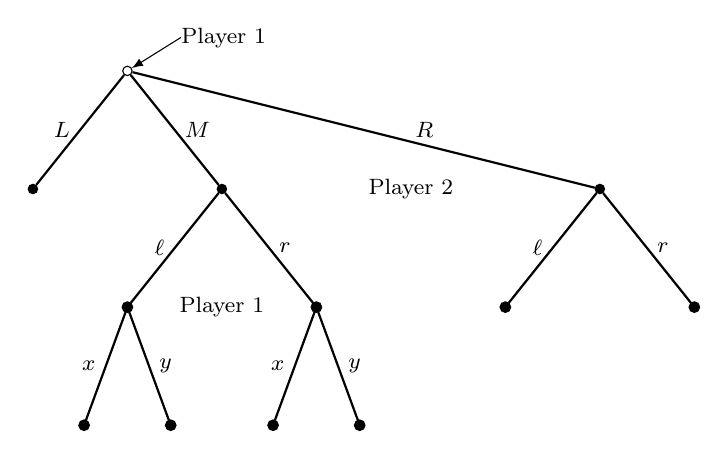
\begin{tikzpicture}[font=\footnotesize,edge from parent/.style={draw,thick}]
% Two node styles: solid and hollow
\tikzstyle{solid node}=[circle,draw,inner sep=1.2,fill=black];
\tikzstyle{hollow node}=[circle,draw,inner sep=1.2];
% Specify spacing for each level of the tree
\tikzstyle{level 1}=[level distance=15mm,sibling distance=12mm]
\tikzstyle{level 2}=[level distance=15mm,sibling distance=24mm]
\tikzstyle{level 3}=[level distance=15mm,sibling distance=11mm]
% The Tree
\node(0)[hollow node]{}
child{node[solid node]{}edge from parent node[left]{$L$}}
child{node[solid node]at +(\tikzsiblingdistance,0){}
child{node[solid node]{}
child{node[solid node]{}edge from parent node[left]{$x$}}
child{node[solid node]{}edge from parent node[right]{$y$}}
edge from parent node[left]{$\ell$}
}
child{node[solid node]{}
child{node[solid node]{}edge from parent node[left]{$x$}}
child{node[solid node]{}edge from parent node[right]{$y$}}
edge from parent node[right]{$r$}
}
edge from parent node[right]{$M$}
}
child[sibling distance=5*\tikzsiblingdistance]{node[solid node]{}
child{node[solid node]{}
edge from parent node[left]{$\ell$}
}
child{node[solid node]{}
edge from parent node[right]{$r$}
}
edge from parent node[right,xshift=15]{$R$}
};
% specifying movers
\draw[draw,<-,>=latex](0)--(32:8mm)node[right,inner sep=0]{Player 1};
\node at ($.5*(0-2)+.5*(0-3)$) {Player 2};
\node at ($.5*(0-2-1)+.5*(0-2-2)$) {Player 1};
\end{tikzpicture}

  \end{figure}
  How many strategies does each player have?
  \begin{choices}
    \choice Player 1: 9 strategies, Player 2: 4 strategies
    \CorrectChoice Player 1: 12 strategies, Player 2: 4 strategies
    \choice Player 1: 7 strategies, Player 2: 2 strategies
    \choice Player 1: 7 strategies, Player 2: 4 strategies
  \end{choices}

  \part Consider the game tree from the previous question.
  Which of the following is a complete strategy profile
  for Player 1?
  \begin{choices}
    \choice $\{ L \}$
    \choice $\{ x \ \text{if} \ \ell \}$
    \CorrectChoice 
      $ \{ L, x \ \text{if} \ \ell,\ y \ \text{if} \ r \} $
    \choice $\{ L, \ x, \ y \}$ 
  \end{choices}

  \part Consider the strategic form game below:
  \begin{table}[h!]
    \begin{center}
    \setlength{\extrarowheight}{2pt}
    \begin{tabular}{*{5}{c|}}
      \multicolumn{2}{c}{} & \multicolumn{3}{c}{$P_2$} \\\cline{3-5}
      \multicolumn{1}{c}{} &     & $x$ & $y$ & $z$ \\\cline{2-5}
      \multirow{3}*{$P_1$}  & $a$ & 1,3 & 2,2 & 3,2 \\\cline{2-5}
                           & $b$ & 2,2 & 2,2 & 4,3 \\\cline{2-5}
                           & $c$ & 1,1 & 0,2 & 1,1 \\\cline{2-5}
    \end{tabular}
    \end{center}
  \end{table}
  In the game above, which strategy is strictly dominated?
  \begin{choices}
    \choice $a$
    \choice $b$ 
    \CorrectChoice $c$
    \choice $x$
  \end{choices}

  \part Perform Iterative Deletion of Strictly Dominated Strategies for the same game as above all the way to completion.
  What does IDSDS tell you about the Nash equilibrium of this game?
  \begin{choices}
    \choice The NE is (a, x)
    \choice The NE is (a, y)
    \choice The NE is (Y, z)
    \CorrectChoice IESDS by itself does not reveal the NE of this game.
  \end{choices}

\end{parts}

\newpage

%------------------------------------------------------------------%

\question[20] 
The countries of Oceania and Eurasia are at war.
As depicted in the figure, Oceania has four cities —
Argula, Betra, Carnat, and Dussel — 
and it is concerned that one of them is to be bombed by Eurasia.
The bombers could come from either base Alpha,
which can reach the cities of Argula and Betra;
or from base Beta, which can reach either Carnat or Dussel.
Eurasia decides which one of these four cities to attack.
Oceania doesn’t know which one has been selected,
but does observe the base from which the bombers are flying.
After making that observation, Oceania decides which one 
(and only one) of its four cities to evacuate.

Assign a payoff of 2 to Oceania
if it succeeds in evacuating the city that is to be bombed
and a payoff of 1 otherwise.
Assign Eurasia a payoff of 1 if the city it bombs was not evacuated
and a zero payoff otherwise.
Write down the extensive form game.
\footnote{Harrington \textit{Games, Strategies, and Decision Making}}

%\vspace{-5cm}
\begin{figure}[!h]
  \centering
  \includegraphics[width=.3\linewidth]{figures/figPR2.1.png} 
\end{figure}

\begin{solution}
  \begin{center}
    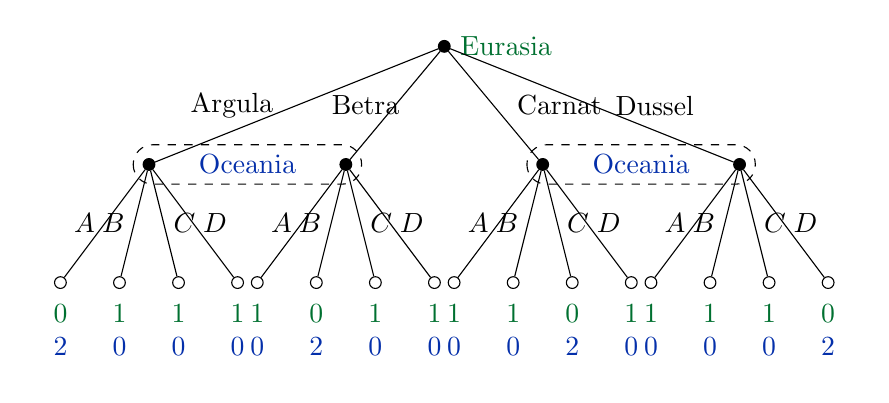
\begin{tikzpicture}[
% font=\footnotesize
]
    \tikzstyle{solid node}=[circle,draw,inner sep=1.5,fill=black]
    \tikzstyle{hollow node}=[circle,draw,inner sep=1.5]
    \tikzstyle{level 1}=[level distance=15mm,sibling distance=2.5cm]
    \tikzstyle{level 2}=[level distance=15mm,sibling distance=.75cm]
    \tikzstyle{level 3}=[level distance=15mm,sibling distance=0.5cm]
    
    \node(0)[solid node,label=right:{\color{ducksgreen} Eurasia}]{}
        child{node(1)[solid node,label=above left:{ }]{}
            child{node[hollow node,label=below:{
                \begin{tabular}{c}
                     {\color{ducksgreen} 0}  \\
                     {\color{darkblue} 2} 
                \end{tabular}
            }]{} edge from parent node[left]{$A$}}
            child{node[hollow node,label=below:{
                \begin{tabular}{c}
                     {\color{ducksgreen} 1}  \\
                     {\color{darkblue} 0} 
                \end{tabular}
            }]{} edge from parent node[left]{$B$}}
            child{node[hollow node,label=below:{
                \begin{tabular}{c}
                     {\color{ducksgreen} 1}  \\
                     {\color{darkblue} 0} 
                \end{tabular}
            }]{} edge from parent node[right]{$C$}}
            child{node[hollow node,label=below:{
                \begin{tabular}{c}
                     {\color{ducksgreen} 1}  \\
                     {\color{darkblue} 0} 
                \end{tabular}
            }]{} edge from parent node[right]{$D$}}
            edge from parent node[left,xshift=-5]{Argula}
        }
        child{node(2)[solid node,label=above right:{ }]{}
            child{node[hollow node,label=below:{
                \begin{tabular}{c}
                     {\color{ducksgreen} 1}  \\
                     {\color{darkblue} 0} 
                \end{tabular}
            }]{} edge from parent node[left]{$A$}}
            child{node[hollow node,label=below:{
                \begin{tabular}{c}
                     {\color{ducksgreen} 0}  \\
                     {\color{darkblue} 2} 
                \end{tabular}
            }]{} edge from parent node[left]{$B$}}
            child{node[hollow node,label=below:{
                \begin{tabular}{c}
                     {\color{ducksgreen} 1}  \\
                     {\color{darkblue} 0} 
                \end{tabular}
            }]{} edge from parent node[right]{$C$}}
            child{node[hollow node,label=below:{
                \begin{tabular}{c}
                     {\color{ducksgreen} 1}  \\
                     {\color{darkblue} 0} 
                \end{tabular}
            }]{} edge from parent node[right]{$D$}}
            edge from parent node[left,xshift=5]{Betra}
        }
        child{node(3)[solid node,label=above right:{ }]{}
            child{node[hollow node,label=below:{
                \begin{tabular}{c}
                     {\color{ducksgreen} 1}  \\
                     {\color{darkblue} 0} 
                \end{tabular}
            }]{} edge from parent node[left]{$A$}}
            child{node[hollow node,label=below:{
                \begin{tabular}{c}
                     {\color{ducksgreen} 1}  \\
                     {\color{darkblue} 0} 
                \end{tabular}
            }]{} edge from parent node[left]{$B$}}
            child{node[hollow node,label=below:{
                \begin{tabular}{c}
                     {\color{ducksgreen} 0}  \\
                     {\color{darkblue} 2} 
                \end{tabular}
            }]{} edge from parent node[right]{$C$}}
            child{node[hollow node,label=below:{
                \begin{tabular}{c}
                     {\color{ducksgreen} 1}  \\
                     {\color{darkblue} 0} 
                \end{tabular}
            }]{} edge from parent node[right]{$D$}}
            edge from parent node[right,xshift=5]{Carnat}
        }
        child{node(4)[solid node,label=above right:{ }]{}
            child{node[hollow node,label=below:{
                \begin{tabular}{c}
                     {\color{ducksgreen} 1}  \\
                     {\color{darkblue} 0} 
                \end{tabular}
            }]{} edge from parent node[left]{$A$}}
            child{node[hollow node,label=below:{
                \begin{tabular}{c}
                     {\color{ducksgreen} 1}  \\
                     {\color{darkblue} 0} 
                \end{tabular}
            }]{} edge from parent node[left]{$B$}}
            child{node[hollow node,label=below:{
                \begin{tabular}{c}
                     {\color{ducksgreen} 1}  \\
                     {\color{darkblue} 0} 
                \end{tabular}
            }]{} edge from parent node[right]{$C$}}
            child{node[hollow node,label=below:{
                \begin{tabular}{c}
                     {\color{ducksgreen} 0}  \\
                     {\color{darkblue} 2} 
                \end{tabular}
            }]{} edge from parent node[right]{$D$}}
            edge from parent node[right,xshift=5]{Dussel}
        };

    % information set
    \draw[dashed,rounded corners=7]($(1)+(-.2,.25)$)rectangle($(2)+(.2,-.25)$);
    \draw[dashed,rounded corners=7]($(3)+(-.2,.25)$)rectangle($(4)+(.2,-.25)$);
    % specify movers
    \node at ($.5*(1)+.5*(2)$) {\color{darkblue} Oceania};
    \node at ($.5*(3)+.5*(4)$) {\color{darkblue} Oceania};
\end{tikzpicture}
 
  \end{center} 

  Note that $A$, $B$, $C$, and $D$ in the last row are short for the city names.
  Eurasia acts first, so the initial node is labelled accordingly.
  Oceania has only two info sets which are represented with the dashed ovals.
  The $(0,2)$ or $(1,0)$ payoff sets correspond to Oceania choosing the same city that is bombed,
  or choosing a different city respectively.
\end{solution}

\newpage


%------------------------------------------------------------------

\question%[20]
Imagine a sequential moves version of rock-paper-scissors
where player 2 gets to pick what they will do after player 1 picks.
Please model the game in its extensive form (as a game tree). 
Assume both player 1 and player 2 only care about the result of the game
and have the following preferences over the result of the game:
win $\succ$ tie $\succ$ loss.
\footnote{Ethan Holdahl, University of Oregon }

\begin{parts}
 
  \part Answer the following questions:
  \begin{subparts}
    \subpart[2] How many nodes are there?
    \subpart[2] How many branches are there?
    \subpart[2] How many terminal nodes are there?
  \end{subparts}

  \part[6] Prune the tree as much as possible. How many branches were you able to eliminate?
    (A complete answer should include your drawing(s) of the game tree)
\end{parts}

\begin{solution}
  \begin{center}
    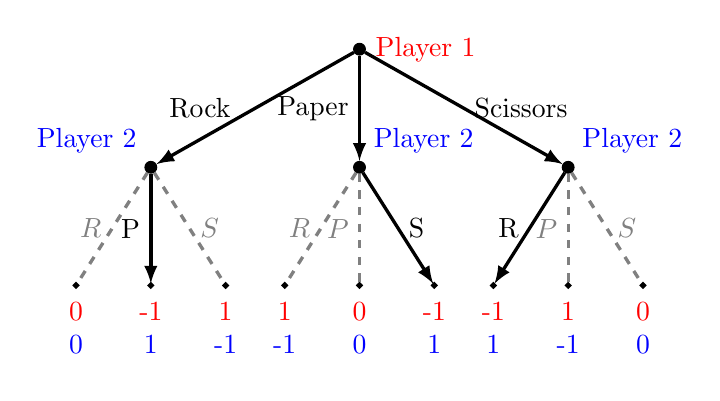
\begin{tikzpicture}[edge from parent/.style={draw, very thick, -latex}]
    \tikzstyle{solid node}=[circle,draw,inner sep=1.5,fill=black]
    \tikzstyle{hollow node}=[circle,draw,inner sep=.25]
    \tikzstyle{level 1}=[level distance=15mm,sibling distance=2.65cm]
    \tikzstyle{level 2}=[level distance=15mm,sibling distance=.95cm]
    \tikzstyle{level 3}=[level distance=15mm,sibling distance=.6cm]
    \tikzstyle{pruned edge from parent}=[draw, very thick, gray, dashed, -]
    
    \node(0)[solid node,label=right:{\color{red} Player 1}]{}
        child{node(1)[solid node,label=above left:{\color{blue} Player 2 }]{}
            child{node[hollow node,label=below:{
                \begin{tabular}{c}
                     {\color{red} 0}  \\
                     {\color{blue} 0} 
                \end{tabular}
            }]{} edge from parent[draw, very thick, gray, dashed, -] node[left]{$R$}}
            child{node[hollow node,label=below:{
                \begin{tabular}{c}
                     {\color{red} -1}  \\
                     {\color{blue} 1} 
                \end{tabular}
            }]{} edge from parent node[left]{P}}
            child{node[hollow node,label=below:{
                \begin{tabular}{c}
                     {\color{red} 1}  \\
                     {\color{blue} -1} 
                \end{tabular}
            }]{} edge from parent[draw, very thick, gray, dashed, -] node[right]{$S$}}
            edge from parent node[left,xshift=-5]{Rock}
        }
        child{node(2)[solid node,label=above right:{\color{blue} Player 2 }]{}
            child{node[hollow node,label=below:{
                \begin{tabular}{c}
                     {\color{red} 1}  \\
                     {\color{blue} -1} 
                \end{tabular}
            }]{} edge from parent[draw, very thick, gray, dashed, -] node[left]{$R$}}
            child{node[hollow node,label=below:{
                \begin{tabular}{c}
                     {\color{red} 0}  \\
                     {\color{blue} 0} 
                \end{tabular}
            }]{} edge from parent[draw, very thick, gray, dashed, -] node[left]{$P$}}
            child{node[hollow node,label=below:{
                \begin{tabular}{c}
                     {\color{red} -1}  \\
                     {\color{blue} 1} 
                \end{tabular}
            }]{} edge from parent node[right]{S}}
            edge from parent node[left]{Paper}
        }
        child{node(3)[solid node,label=above right:{\color{blue} Player 2 }]{}
            child{node[hollow node,label=below:{
                \begin{tabular}{c}
                     {\color{red} -1}  \\
                     {\color{blue} 1} 
                \end{tabular}
            }]{} edge from parent node[left]{R}}
            child{node[hollow node,label=below:{
                \begin{tabular}{c}
                     {\color{red} 1}  \\
                     {\color{blue} -1} 
                \end{tabular}
            }]{} edge from parent[draw, very thick, gray, dashed, -] node[left]{$P$}}
            child{node[hollow node,label=below:{
                \begin{tabular}{c}
                     {\color{red} 0}  \\
                     {\color{blue} 0} 
                \end{tabular}
            }]{} edge from parent[draw, very thick, gray, dashed, -] node[right]{$S$}}
            edge from parent node[right]{Scissors}
        };
\end{tikzpicture}

  \end{center}
  
  In the figure, dashed lines represent those which have been pruned.

  The tree has 4 nodes, 12 branches, and 9 terminal nodes.

  In each of Player 2's subgames,
  we can prune the two branches where they would lose or times
  based on what Player 1 chose.
  We can't prune any more branches
  because Player 1 is indifferent between all outcomes where they lose.
\end{solution}

\newpage

Use the same setup, but now imagine player 1's preferences change
because they want to be seen as a "tough guy".
Given that what they want to play remains the same,
they still have the following preferences over the result of the game:
win $\succ$ tie $\succ$ loss.
However, they now would prefer to lose playing rock
than win playing paper or scissors. 
Please create a new game tree so the payoffs reflect these new preferences.

\begin{parts}
  \part[8] Prune the tree as much as possible. 
  How many branches were you able to eliminate?
    (Include your drawing(s))
\end{parts}

\begin{solution}
  \begin{center}
    \include{figures/rockpaperscissors2}
  \end{center}

  I represented Player 1's preferences as:

  payoff to winning with rock = 4,
  tie with rock = 3, 
  lose with rock = 2,
  win with paper or scissors = 1,
  tie with paper or scissors = 0,
  lose with paper or scissors = -1.

  Because payoffs are \textit{ordinal}, 
  you can choose any values as long as the ranking is the same.

  Now because Player 1 prefers to lose with rock to any other loss, 
  we can prune the branches where they choose either 
  paper or scissors.
  
  The rollback solution is 
  \{ Player 1 chooses Rock, 
  (Player 2 chooses paper if rock,
  scissors if paper,
  and rock if scissors) \}.
   
\end{solution}

\newpage

%------------------------------------------------------------------

\question%[20]
Here's a little ditty, about Jack and Diane,
two American kids growing up in the heartland.
The game is below.
\footnote{Cliff Bekar, Lewis and Clark College}

  \begin{table}[h!]
    \centering
    \setlength{\extrarowheight}{2pt}
    \begin{tabular}{*{5}{c|}}
      \multicolumn{2}{c}{} & \multicolumn{3}{c}{Diane} \\\cline{3-5}
      \multicolumn{1}{c}{} &     & $x$ & $y$ & $z$ \\\cline{2-5}
      \multirow{3}*{Jack}  & $a$ & 1,1 & 2,1 & 2,0 \\\cline{2-5}
                           & $b$ & 2,3 & 0,2 & 2,1 \\\cline{2-5}
                           & $c$ & 2,1 & 1,2 & 3,0 \\\cline{2-5}
    \end{tabular}
  \end{table}

\begin{parts}
  \part[8] Find all pure Nash strategy profiles and outcomes 
    if Jack and Diane move simultaneously.
    Carefully detail and explain your strategy profiles 
    and how they map onto your Nash outcomes. 
    \part[12] Find all pure Nash strategy profiles and outcomes
    if Jack moves first.
    Carefully detail and explain your strategy profiles 
    and how they map onto your Nash outcomes.
\end{parts}

\newpage


%------------------------------------------------------------------

\question%[20]
See the figures below for the data from our in-class activity 2 
\footnote{You can also find the data on Canvas in the \textit{Activities} folder of the \textit{files} tab}.
where teams took turns taking flags from a starting pool. 
Note that in Game 1,
6 out of 9 matches were won by the first team to take flags 
and in Game 2, 3 of 9 matches were won by the starting team.

\begin{parts}
  \part[10] Using the rollback equilibrium as a predictive model,
  how many times would you expect the starting team to win 
  when all agents are \textit{perfectly informed}, \textit{rational},
  and have \textit{common knowledge of rationality}?
  Based on the class data, should we \textit{accept} or \textit{reject}
  this hypothesis?

  \part[10] Based on your observations in class 
  and the results from other groups, 
  which of the assumptions above do you think could be modified
  to create a more accurate model of this game?
  What modifications would you make,
  and what alternative hypotheses could you test?

\end{parts}

\newpage 

\begin{figure}[!h]
  \centering
  \includegraphics[width=.6\linewidth]{figures/Game1.png} 
\end{figure}

\begin{figure}[!h]
  \centering
  \includegraphics[width=.6\linewidth]{figures/Game2.png} 
\end{figure}


%------------------------------------------------------------------

\end{questions}

\end{document}
